\chapter*{Einleitung}

In der Industrie gewinnt Vernetzbarkeit immer mehr Bedeutung. Auch das Vernetzen von externen Geräten mit den Produktions-Maschinen wird immer gebräuchlicher, um die Arbeitseffizienz zu erhöhen. Um diese Kommunikation zu vereinfachen und verbessern wurde das Process Field Network (im Folgenden \gls{profinet}) entwickelt.\\
\gls{profinet} setzt auf Ethernet für echtzeitfähige Anwendungen und \gls{tcp}/\gls{ip} für langsamere \gls{io} Anwendungen. Durch die immer mehr vernetzten und oft dem Internet zugänglichen Produktionsstätten ist Sicherheit mittlerweile von höchster Bedeutung. \\
Dieses Projekt setzt an dieser Stelle an und soll dem \gls{ids} \gls{snort} ermöglichen, die \gls{profinet} Protokolle zu verstehen und zu verarbeiten. Um dem Benutzer eine Übersicht über die stattfindenden Kommunikationsprozesse zu verschaffen, soll eine \gls{gui} entwickelt werden. Diese soll mithilfe verschiedener Graphalgorithmen eine geordnete Darstellung ermöglichen.

\begin{figure}
  \centering
  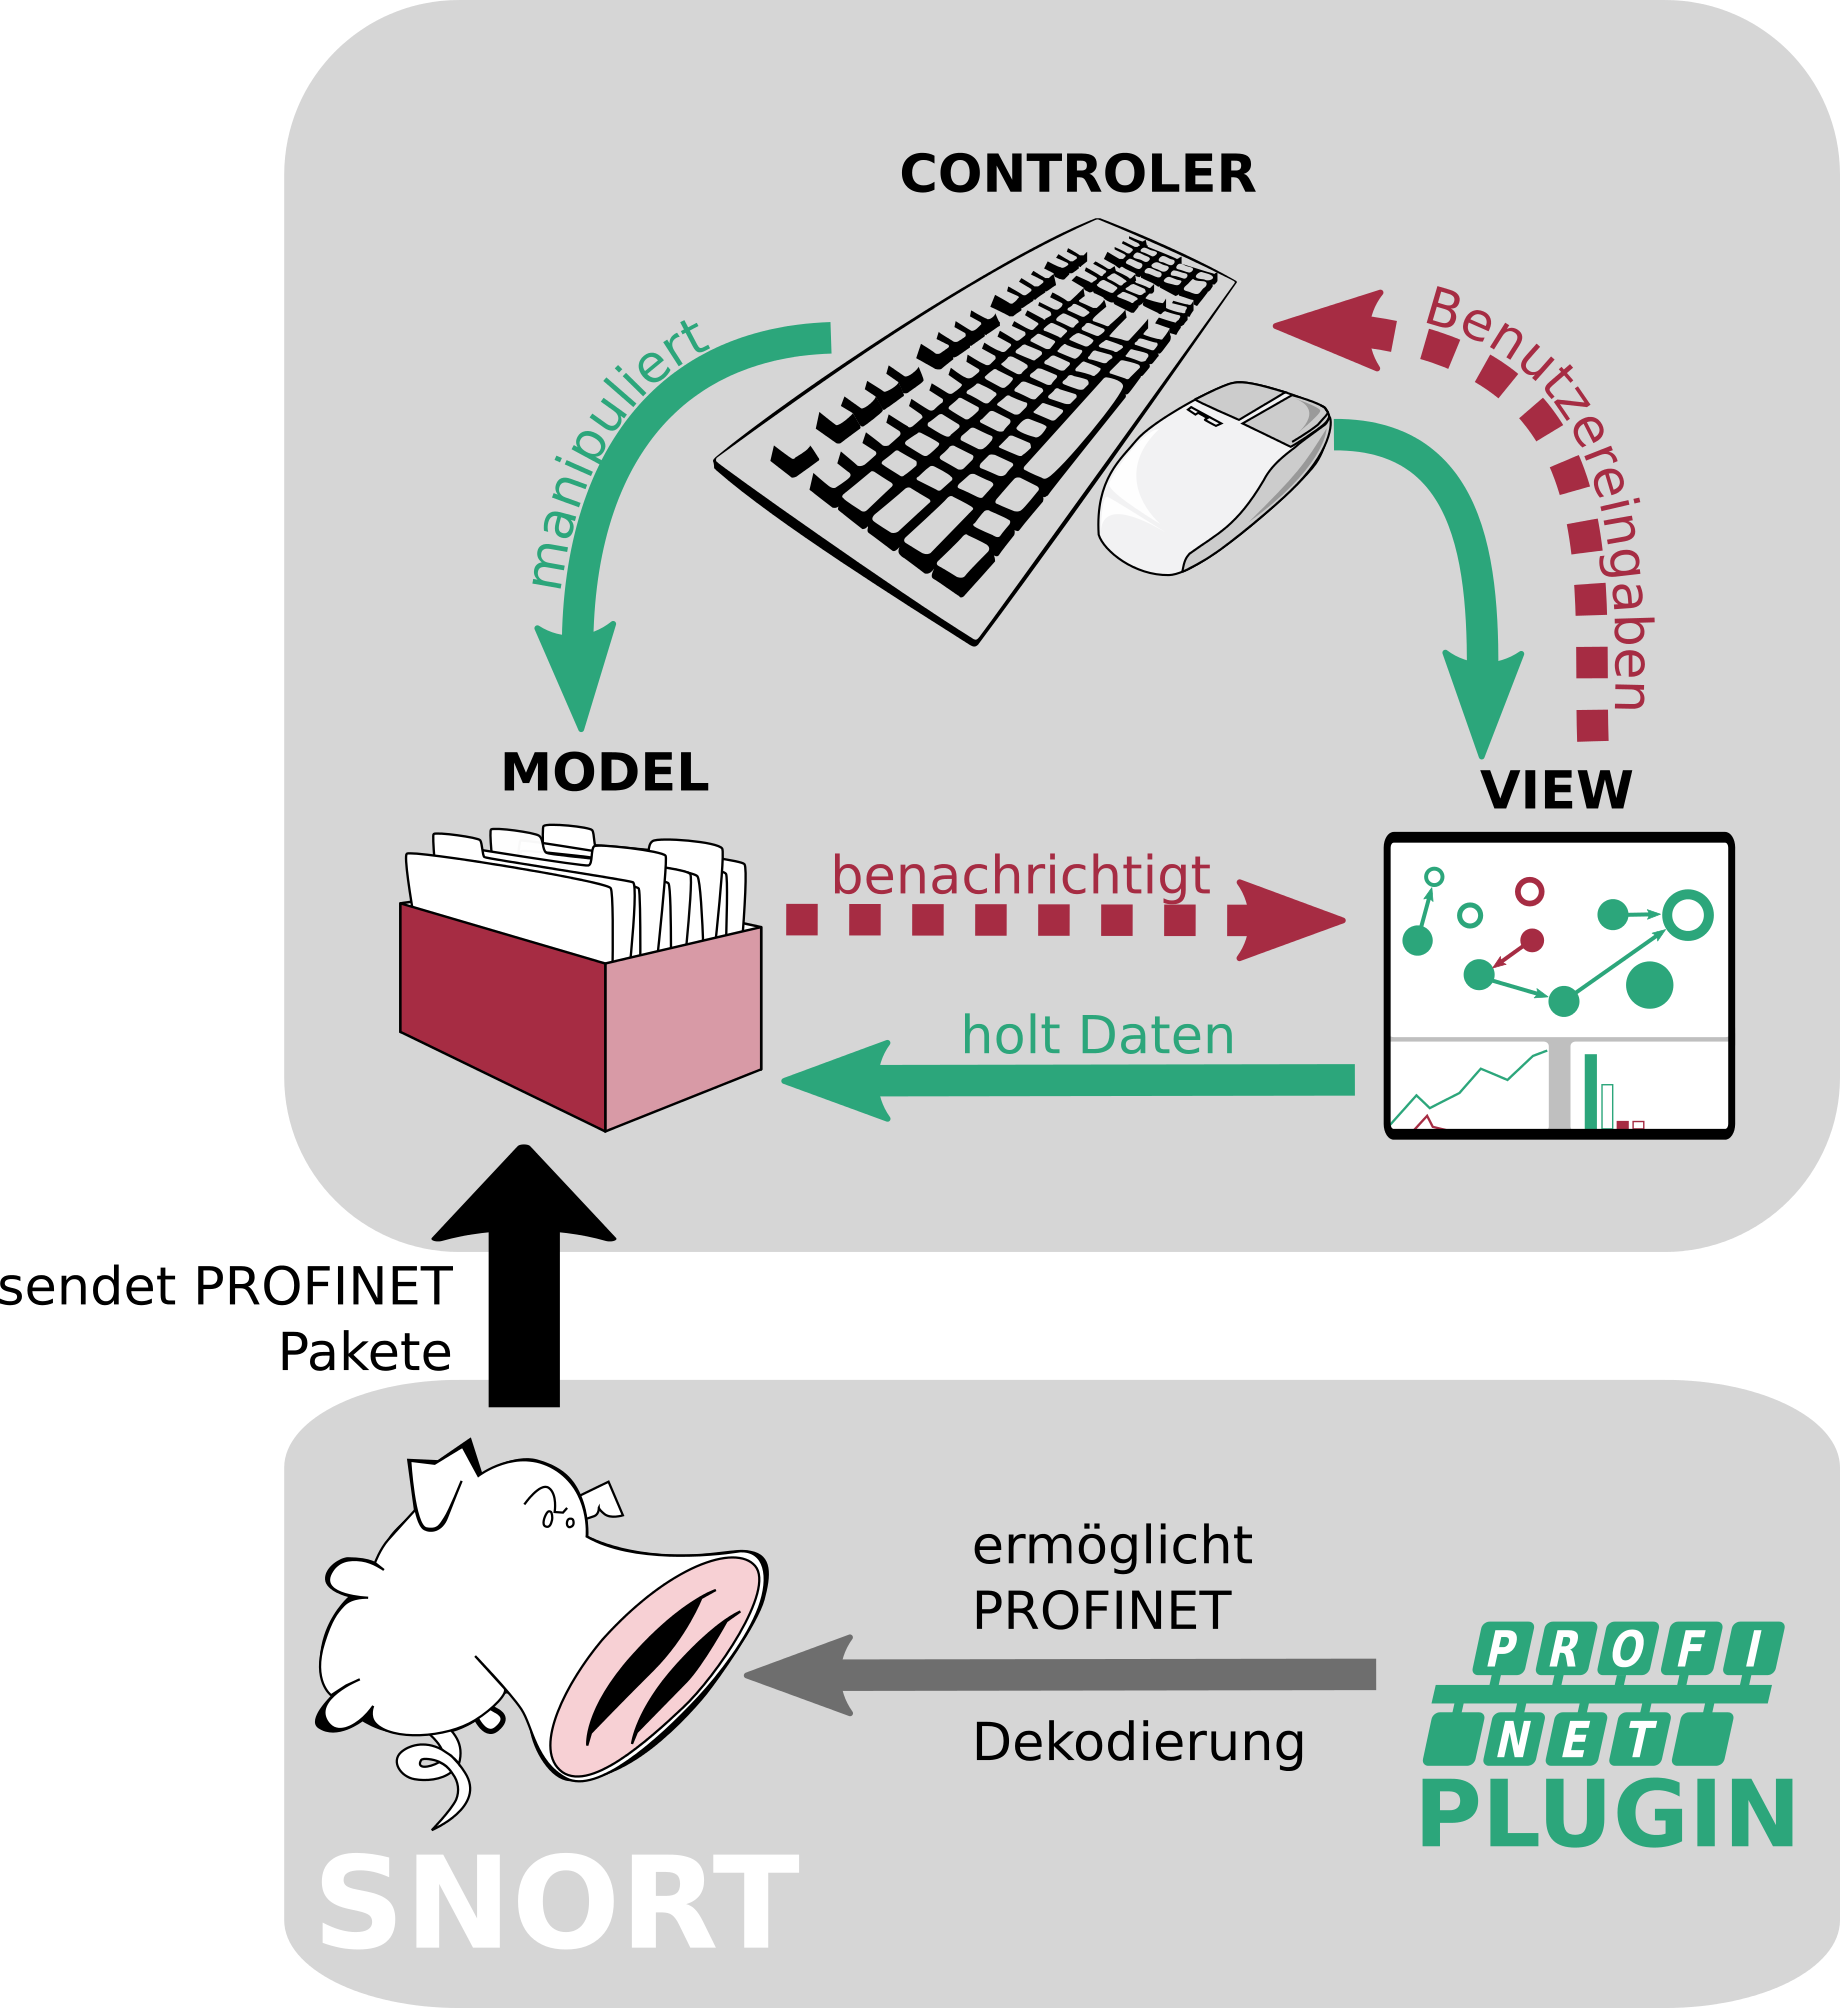
\includegraphics[width=\textwidth]{../diagrams/intro_diagram/g5171.png}
  \caption{Strukturübersicht des Projekts}\label{ASDF}
\end{figure} 